\section{Data Description and EDA}


We summarized the dataset's key statistics to identify trends, central tendencies, and potential anomalies in the data.
Descriptive summaries provided insights into the distribution of 
demographic, clinical, and hospitalization-related variables.

\textcolor{red}{table and figures in appendix}

Many of the numerical variables exhibited significant skewness and the presence of outliers.

\begin{itemize}
    \item \textbf{Shapiro-Wilk Test:} This test confirmed that nearly all variables deviated significantly from normality.
    \item \textbf{Skewness and Kurtosis:} These measures indicated that several variables had heavy-tailed distributions. This finding suggested the need for scaling and normalization techniques to ensure reliable modeling.
\end{itemize}

To explore inter-variable relationships and assess the risk of multicollinearity,
 we performed a correlation analysis across the dataset. 
The results(Figure \ref{fig:correlation_matrix}) identified strong linear relationships among several variable groups:

\begin{figure}[!h]
    \centering
    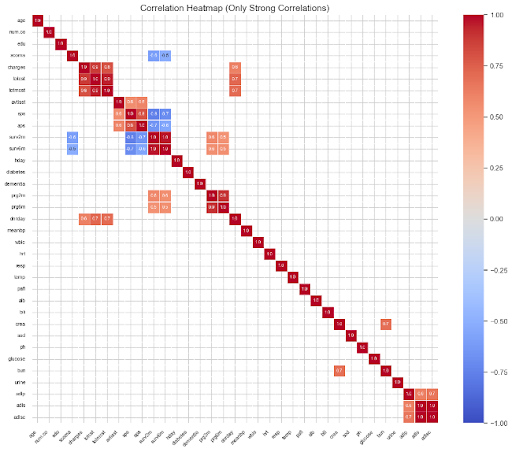
\includegraphics[width=0.8\textwidth]{../results/correlation_target.png}
    \caption{Correlation matrix of the SUPPORT2 dataset.}
    \label{fig:correlation_matrix}
\end{figure}

\begin{itemize}
    \item \textbf{Medical Cost Variables:} \texttt{charges}, \texttt{totcst}, and \texttt{totmcst} showed high positive correlations.
    \item \textbf{Physiological Measures:} \texttt{aps}, \texttt{sps}, and \texttt{avtisst} demonstrated strong internal correlations.
    \item \textbf{Survival Probabilities:} \texttt{surv2m}, \texttt{surv6m}, \texttt{prg2m}, and \texttt{prg6m} were highly correlated, suggesting they reflect overlapping prognostic information.
    \item \textbf{Activities of Daily Living (ADL):} \texttt{adlp}, \texttt{adls}, and \texttt{adlsc} were also strongly related.
\end{itemize}

Understanding the distribution of our target variable \texttt{sfdm2} is crucial for selecting appropriate modeling approaches and evaluation metrics. SFDM2 quantifies patient functional disability on a 1--5 severity scale, with 5 representing maximum impairment. This metric was derived from Sickness 
Impact Profile (SIP) questionnaires via patients and/or their surrogates to systematically evaluate functional status.

\begin{table}[H]
    \centering
    \renewcommand{\arraystretch}{1.5} % Optional: adds vertical padding
    \caption{SFDMS Category Descriptions}
    \begin{tabular}{|M{1.5cm}|M{4cm}|M{7cm}|}
    \hline
    \textbf{Level} & \textbf{Class Name} & \textbf{Meanings} \\
    \hline
    1 & no (Month 2 \& SIP present) & No signs of moderate to severe functional disability. \\
    \hline
    2 & adl $\geq$ 4 ($\geq$ 5 if survived) & Patient was unable to do 4 or more activities of daily living. \\
    \hline
    3 & SIP $\geq$ 30 & Sickness Impact Profile total score at 2 months is greater or equal to 30. \\
    \hline
    4 & Coma or Intubated & Patient intubated or in coma. \\
    \hline
    5 & $<$ 2 mo. follow-up & Patient died before 2 months after study entry. \\
    \hline
    \end{tabular}
\end{table}

The proportion of 5 different target values in response variable is shown in Figure\ref{fig:train_test_target_proportion}.
This imbalance necessitates careful consideration during model development, 
potentially requiring techniques such as resampling,class weighting, or specialized algorithms.

\textcolor{red}{figure in appendix}